\documentclass[border=3mm]{standalone}
\usepackage{tikz}
\usetikzlibrary{arrows, shapes.gates.logic.US, shapes.gates.logic.IEC, calc}

\tikzset{
    my-nand-gate/.style={
        nand gate US, draw, rotate=0, logic gate inputs=nn
    },
    my-branch/.style={
        fill, shape=circle, minimum size=3pt, inner sep=0pt
    },
    my-not-gate/.style={
        not gate US, draw, rotate=-90, logic gate inputs=nn
    },
}

\begin{document}

\resizebox{16cm}{!}{

    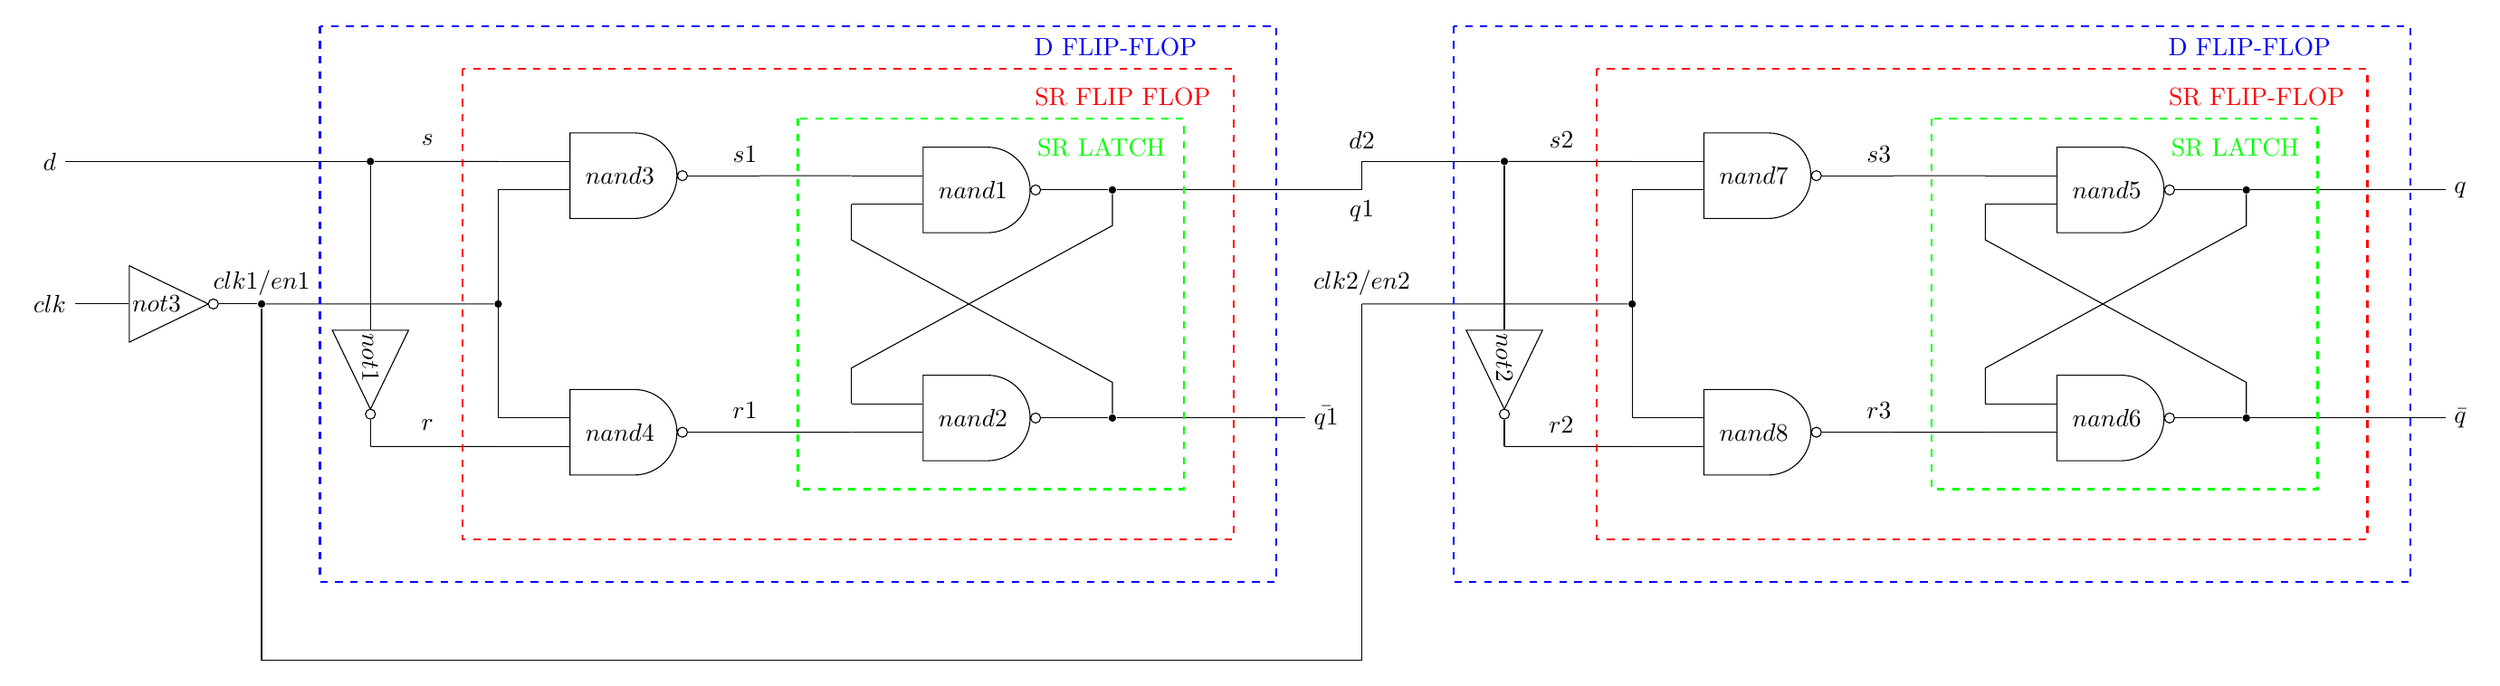
\begin{tikzpicture}[label distance=2mm]

        % INPUT AND CLOCK ------------------------------------------------------------------

        % INPUTS
        \node[] (D)   at (0,0) {\normalsize $d$};
        \node[] (CLK) at ($(D) + (0, -2)$) {\normalsize $clk$};

        % INPUT COORDINATES
        \node[my-branch] (S) at ($(D) + (4.5, 0)$) {};
        \coordinate[]    (R) at ($(D) + (4.5, -4)$) {};

        % NOT3
        \node[my-not-gate, rotate=90] (NOT3) at ($(CLK) + (1.5, 0)$) {\normalsize $not3$};
        \coordinate[]      (NOT3IN1) at ($(NOT3.input)  + (-.5, 0)$)  {};
        \coordinate[]      (NOT3OUT) at ($(NOT3.output) + (.5, 0)$) {};
        \draw (NOT3.input)  -- (NOT3IN1);
        \draw (NOT3.output) -- (NOT3OUT);

        % CLOCK BRANCH
        \node[my-branch] (CLK1) at ($(NOT3OUT) + (.1, 0)$) {};
        \node at ($(CLK1) + (0, .3)$) {\normalsize $clk1/en1$};

        % CLOCK CONNECTIONS (MORE AT END)
        \draw (CLK) -- (NOT3IN1);
        \draw (NOT3OUT) -- (CLK1);
        \coordinate[] (CLKNODE1) at ($(CLK1) + (0, -5)$) {};
        \draw (CLK1) -- (CLKNODE1);

        % MASTER ------------------------------------------------------------------

        % NAND3, WIRES AND CONNECTOR POINTS
        \node[my-nand-gate] (NAND3)    at ($(S) + (3.5, -.2)$)            {\normalsize $nand3$};
        \coordinate[]       (NAND3IN1) at ($(NAND3.input 1) + (-1, 0)$) {};
        \coordinate[]       (NAND3IN2) at ($(NAND3.input 2) + (-1, 0)$) {};
        \coordinate[]       (NAND3OUT) at ($(NAND3.output)  + (1, 0)$)  {};
        \draw (NAND3.input 1) -- (NAND3IN1);
        \draw (NAND3.input 2) -- (NAND3IN2);
        \draw (NAND3.output)  -- (NAND3OUT);
        
        % NAND4, WIRES AND CONNECTOR POINTS
        \node[my-nand-gate] (NAND4)    at ($(R) + (3.5, .2)$)             {\normalsize $nand4$};
        \coordinate[]       (NAND4IN1) at ($(NAND4.input 1) + (-1, 0)$) {};
        \coordinate[]       (NAND4IN2) at ($(NAND4.input 2) + (-1, 0)$) {};
        \coordinate[]       (NAND4OUT) at ($(NAND4.output)  + (1, 0)$)  {};
        \draw (NAND4.input 1) -- (NAND4IN1);
        \draw (NAND4.input 2) -- (NAND4IN2);
        \draw (NAND4.output)  -- (NAND4OUT);

        % NAND1, WIRES AND CONNECTOR POINTS
        \node[my-nand-gate] (NAND1)    at ($(NAND3OUT) + (3, -.2)$)     {\normalsize $nand1$};
        \coordinate[]       (NAND1IN1) at ($(NAND1.input 1) + (-1, 0)$) {};
        \coordinate[]       (NAND1IN2) at ($(NAND1.input 2) + (-1, 0)$) {};
        \node[my-branch]    (NAND1OUT) at ($(NAND1.output)  + (1, 0)$)  {};
        \draw (NAND1.input 1) -- (NAND1IN1);
        \draw (NAND1.input 2) -- (NAND1IN2);
        \draw (NAND1.output)  -- (NAND1OUT);
        
        % NAND2, WIRES AND CONNECTOR POINTS
        \node[my-nand-gate] (NAND2)    at ($(NAND4OUT) + (3, .2)$)      {\normalsize $nand2$};
        \coordinate[]       (NAND2IN1) at ($(NAND2.input 1) + (-1, 0)$) {};
        \coordinate[]       (NAND2IN2) at ($(NAND2.input 2) + (-1, 0)$) {};
        \node[my-branch]    (NAND2OUT) at ($(NAND2.output)  + (1, 0)$)  {};
        \draw (NAND2.input 1) -- (NAND2IN1);
        \draw (NAND2.input 2) -- (NAND2IN2);
        \draw (NAND2.output)  -- (NAND2OUT);

        % NOT1
        \node[my-not-gate]  (NOT1)    at ($(S) + (0, -2.75)$)    {\normalsize $not1$};
        \coordinate[] (NOT1IN1) at ($(NOT1.input)  + (0, .25)$)  {};
        \coordinate[] (NOT1OUT) at ($(NOT1.output) + (0, -.25)$) {};
        \draw (NOT1.input)  -- (NOT1IN1);
        \draw (NOT1.output) -- (NOT1OUT);

        % OUTPUTS
        \coordinate[] (Q1) at ($(NAND1OUT) + (3.5, 0)$) {};
        \node at ($(Q1) + (0, -.3)$) {\normalsize $q1$};
        \node[] (Q1BAR) at ($(NAND2OUT) + (3, 0)$) {\normalsize $\bar{q1}$};
                
        % INPUT CONNECTIONS
        \draw (D) -- (S);
        \draw (S) -- (NOT1IN1);
        \draw (NOT1OUT) -- (R);
        \node at ($(S) + (.8, .3)$) {\normalsize $s$};
        \draw (S) -- (NAND3IN1);
        \draw (R) -- (NAND4IN2);
        \node at ($(R) + (.8, .3)$) {\normalsize $r$};
        
        % OUTPUT CONNECTIONS
        \draw (NAND1OUT) -- (Q1);
        \draw (NAND2OUT) -- (Q1BAR);

        % INTERNAL WIRES - NAND GATES
        \draw (NAND3OUT) -- (NAND1IN1) node[pos=0] (S1) {};
        \node at ($(S1) + (-.2, .3)$) {\normalsize $s1$};
        \draw (NAND4OUT) -- (NAND2IN2) node[pos=0] (R1) {};
        \node at ($(R1) + (-.2, .3)$) {\normalsize $r1$};
        \draw (NAND1OUT) -- ++(0,-0.5) -- ($(NAND2IN1) +(0,0.5)$)  -- (NAND2IN1);
        \draw (NAND2OUT) -- ++(0,0.5)  -- ($(NAND1IN2) +(0,-0.5)$) -- (NAND1IN2);

        % INTERNAL WIRES - CLOCK
        \draw (NAND3IN2) -- (NAND4IN1) node[my-branch, pos=1/2] (CLKBRANCH) {};
        \draw (CLK1) -- (CLKBRANCH);

        % DRAW DOTTED LINE BOX AROUND SR LATCH
        \draw[thick, dashed, green] ($(NAND1IN1) + (-.75, .8)$) rectangle ($(NAND2OUT) + (1, -1)$);
        \node[green] at ($(NAND1) + (1.8, .6)$) {\normalsize SR LATCH};

        % DRAW DOTTED LINE BOX AROUND SR FLIP-FLOP
        \draw[thick, dashed, red] ($(NAND3IN1) + (-.5, 1.3)$) rectangle ($(NAND2OUT) + (1.7, -1.7)$);
        \node[red] at ($(NAND1) + (2.1, 1.3)$) {\normalsize SR FLIP FLOP};

        % DRAW DOTTED LINE BOX AROUND D FLIP-FLOP
        \draw[thick, dashed, blue] ($(NAND3IN1) + (-2.5, 1.9)$) rectangle ($(NAND2OUT) + (2.3, -2.3)$);
        \node[blue] at ($(NAND1) + (2, 2)$) {\normalsize D FLIP-FLOP};
        
        % SLAVE ------------------------------------------------------------------

        % INPUTS
        \coordinate[] (D2)  at ($(Q1) + (0, .4)$) {};
        \node at ($(D2) + (0, .3)$) {\normalsize $d2$};
        \coordinate[] (CLK2) at ($(D2) + (0, -2)$) {};
        \node at ($(CLK2) + (0, .3)$) {\normalsize $clk2/en2$};

        % INPUT COORDINATES
        \node[my-branch] (S2) at ($(D2) + (2, 0)$)  {};
        \coordinate[]    (R2) at ($(D2) + (2, -4)$) {};

        % NAND7, WIRES AND CONNECTOR POINTS
        \node[my-nand-gate] (NAND7)    at ($(S2) + (3.5, -.2)$)         {\normalsize $nand7$};
        \coordinate[]       (NAND7IN1) at ($(NAND7.input 1) + (-1, 0)$) {};
        \coordinate[]       (NAND7IN2) at ($(NAND7.input 2) + (-1, 0)$) {};
        \coordinate[]       (NAND7OUT) at ($(NAND7.output)  + (1, 0)$)  {};
        \draw (NAND7.input 1) -- (NAND7IN1);
        \draw (NAND7.input 2) -- (NAND7IN2);
        \draw (NAND7.output)  -- (NAND7OUT);
        
        % NAND8, WIRES AND CONNECTOR POINTS
        \node[my-nand-gate] (NAND8)    at ($(R2) + (3.5, .2)$)       {\normalsize $nand8$};
        \coordinate[]       (NAND8IN1) at ($(NAND8.input 1) + (-1, 0)$) {};
        \coordinate[]       (NAND8IN2) at ($(NAND8.input 2) + (-1, 0)$) {};
        \coordinate[]       (NAND8OUT) at ($(NAND8.output)  + (1, 0)$)  {};
        \draw (NAND8.input 1) -- (NAND8IN1);
        \draw (NAND8.input 2) -- (NAND8IN2);
        \draw (NAND8.output)  -- (NAND8OUT);

        % NAND5, WIRES AND CONNECTOR POINTS
        \node[my-nand-gate] (NAND5)    at ($(NAND7OUT) + (3, -.2)$)     {\normalsize $nand5$};
        \coordinate[]       (NAND5IN1) at ($(NAND5.input 1) + (-1, 0)$) {};
        \coordinate[]       (NAND5IN2) at ($(NAND5.input 2) + (-1, 0)$) {};
        \node[my-branch]    (NAND5OUT) at ($(NAND5.output)  + (1, 0)$)  {};
        \draw (NAND5.input 1) -- (NAND5IN1);
        \draw (NAND5.input 2) -- (NAND5IN2);
        \draw (NAND5.output)  -- (NAND5OUT);
        
        % NAND6, WIRES AND CONNECTOR POINTS
        \node[my-nand-gate] (NAND6)    at ($(NAND8OUT) + (3, .2)$)      {\normalsize $nand6$};
        \coordinate[]       (NAND6IN1) at ($(NAND6.input 1) + (-1, 0)$) {};
        \coordinate[]       (NAND6IN2) at ($(NAND6.input 2) + (-1, 0)$) {};
        \node[my-branch]    (NAND6OUT) at ($(NAND6.output)  + (1, 0)$)  {};
        \draw (NAND6.input 1) -- (NAND6IN1);
        \draw (NAND6.input 2) -- (NAND6IN2);
        \draw (NAND6.output)  -- (NAND6OUT);

        % NOT2
        \node[my-not-gate] (NOT2)    at ($(S2) + (0, -2.75)$)         {\normalsize $not2$};
        \coordinate[]      (NOT2IN1) at ($(NOT2.input)  + (0, .25)$)  {};
        \coordinate[]      (NOT2OUT) at ($(NOT2.output) + (0, -.25)$) {};
        \draw (NOT2.input)  -- (NOT2IN1);
        \draw (NOT2.output) -- (NOT2OUT);

        % OUTPUTS
        \node[] (Q)    at ($(NAND5OUT) + (3, 0)$) {\normalsize $q$};
        \node[] (QBAR) at ($(NAND6OUT) + (3, 0)$) {\normalsize $\bar{q}$};

        % INPUT CONNECTIONS
        \draw (D2) -- (S2);
        \draw (S2) -- (NOT2IN1);
        \draw (NOT2OUT) -- (R2);
        \node at ($(S2) + (.8, .3)$) {\normalsize $s2$};
        \draw (S2) -- (NAND7IN1);
        \draw (R2) -- (NAND8IN2);
        \node at ($(R2) + (.8, .3)$) {\normalsize $r2$};
        
        % OUTPUT CONNECTIONS
        \draw (NAND5OUT) -- (Q);
        \draw (NAND6OUT) -- (QBAR);

        % INTERNAL WIRES - NAND GATES
        \draw (NAND7OUT) -- (NAND5IN1) node[pos=0] (S3) {};
        \node at ($(S3) + (-.2, .3)$) {\normalsize $s3$};
        \draw (NAND8OUT) -- (NAND6IN2) node[pos=0] (R3) {};
        \node at ($(R3) + (-.2, .3)$) {\normalsize $r3$};
        \draw (NAND5OUT) -- ++(0,-0.5) -- ($(NAND6IN1) + (0,0.5)$)  -- (NAND6IN1);
        \draw (NAND6OUT) -- ++(0,0.5)  -- ($(NAND5IN2) + (0,-0.5)$) -- (NAND5IN2);

        % INTERNAL WIRES - CLOCK
        \draw (NAND7IN2) -- (NAND8IN1) node[my-branch, pos=1/2] (CLK2BRANCH) {};
        \draw (CLK2) -- (CLK2BRANCH);

        % DRAW DOTTED LINE BOX AROUND SR LATCH
        \draw[thick, dashed, green] ($(NAND5IN1) + (-.75, .8)$) rectangle ($(NAND6OUT) + (1, -1)$);
        \node[green] at ($(NAND5) + (1.8, .6)$) {\normalsize SR LATCH};

        % DRAW DOTTED LINE BOX AROUND SR FLIP-FLOP
        \draw[thick, dashed, red] ($(NAND7IN1) + (-.5, 1.3)$) rectangle ($(NAND6OUT) + (1.7, -1.7)$);
        \node[red] at ($(NAND5) + (2.1, 1.3)$) {\normalsize SR FLIP-FLOP};
        
        % DRAW DOTTED LINE BOX AROUND D FLIP-FLOP
        \draw[thick, dashed, blue] ($(NAND7IN1) + (-2.5, 1.9)$) rectangle ($(NAND6OUT) + (2.3, -2.3)$);
        \node[blue] at ($(NAND5) + (2, 2)$) {\normalsize D FLIP-FLOP};

        % CONNECT D FLIP-FLOPS ------------------------------------------------------------

        % CONNECT FLIP-FLOPS
        \draw (Q1) -- (D2);

        % CLOCK CONNECTIONS (MORE AT TOP)
        \coordinate[] (CLKNODE2) at ($(CLK2) + (0, -5)$) {};
        \draw (CLK2) -- (CLKNODE2);
        \draw (CLKNODE1) -- (CLKNODE2);

    \end{tikzpicture}
}

\end{document} 
